% Copyright © 2015 Martin Ueding <dev@martin-ueding.de>

\documentclass[11pt, english, fleqn, DIV=15, headinclude, BCOR=1cm]{scrartcl}

\usepackage[bibatend, color]{../header}

\usepackage{tikz}

\usepackage[tikz]{mdframed}
\newmdtheoremenv[%
    backgroundcolor=black!5,
    innertopmargin=\topskip,
    splittopskip=\topskip,
]{theorem}{Theorem}[section]

\hypersetup{
    pdftitle=
}

\newcounter{totalpoints}
\newcommand\punkte[1]{#1\addtocounter{totalpoints}{#1}}

\newcounter{problemset}
\setcounter{problemset}{1}

\subject{Geometry in Physics}
\ihead{Geometry in Physics -- Problem Set \arabic{problemset}}

\title{Problem Set \arabic{problemset}}

\publishers{Group 1}
\ofoot{Group 1}

\author{
    Martin Ueding \\ \small{\href{mailto:mu@martin-ueding.de}{mu@martin-ueding.de}}
    \and
    Paul Manz \\ \small{\href{mailto:paul.manz@dreiacht.de}{paul.manz@dreiacht.de}}
}
\ifoot{Martin Ueding, Paul Manz}

\ohead{\rightmark}

\usepackage{multicol}

\begin{document}

\maketitle

\vspace{3ex}

\begin{center}
    \begin{tabular}{rrr}
        problem number & achieved points & possible points \\
        \midrule
        1 & & \punkte{30} \\
        2 & & \punkte{20} \\
        \midrule
        Total & & \arabic{totalpoints}
    \end{tabular}
\end{center}

\vspace{5ex}

I, Martin Ueding, would like to scan and upload the problem sets with your
corrections to my website \href{http://martin-ueding.de}{martin-ueding.de}.
There, the original problem set as well as the reviewed one will be licensed
under the “\href{http://creativecommons.org/licenses/by-sa/4.0/}{Creative
Commons Attribution-ShareAlike 4.0 International License}”. Is that okay with
you?

Yes $\Box$ \hspace{2cm} No $\Box$

\newpage

\section{Differentiable Structure of $S^2$}

\subsection{Domain and image}

The domains and images are shown in Figure~\ref{fig:domains}. They have to be
open, so the boundary must not be included. The image is always the open unit
disk, which is just a unit circle. The unit circle itself is a subset of
$\R^2$, we show it embedded in $\R^3$ because the definition given in
Equation~(1) on the problem set writes the mapping as a $\R^3 \to \R^3$
mapping.

\begin{figure}[htbp]
    \centering
    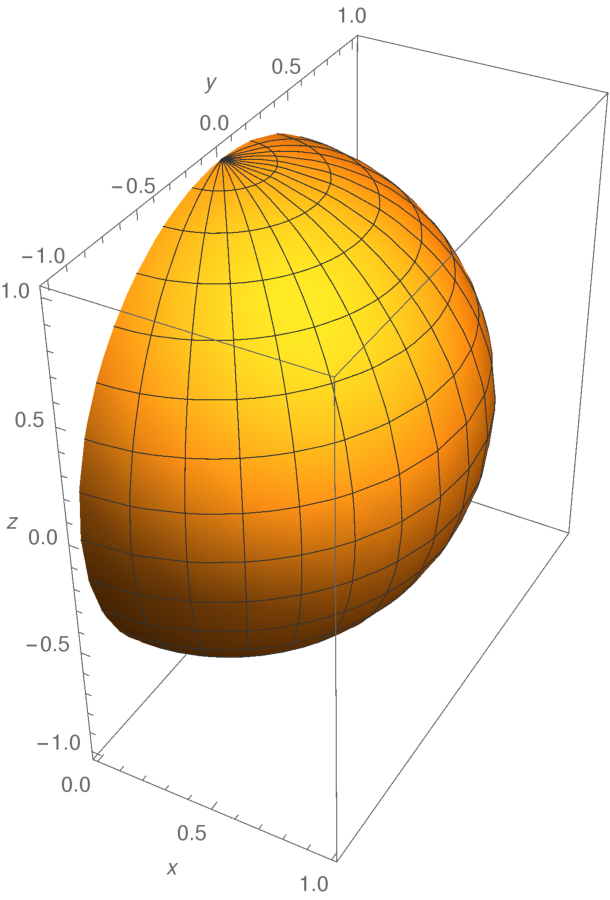
\includegraphics[width=.3\linewidth]{x-plus.pdf}
    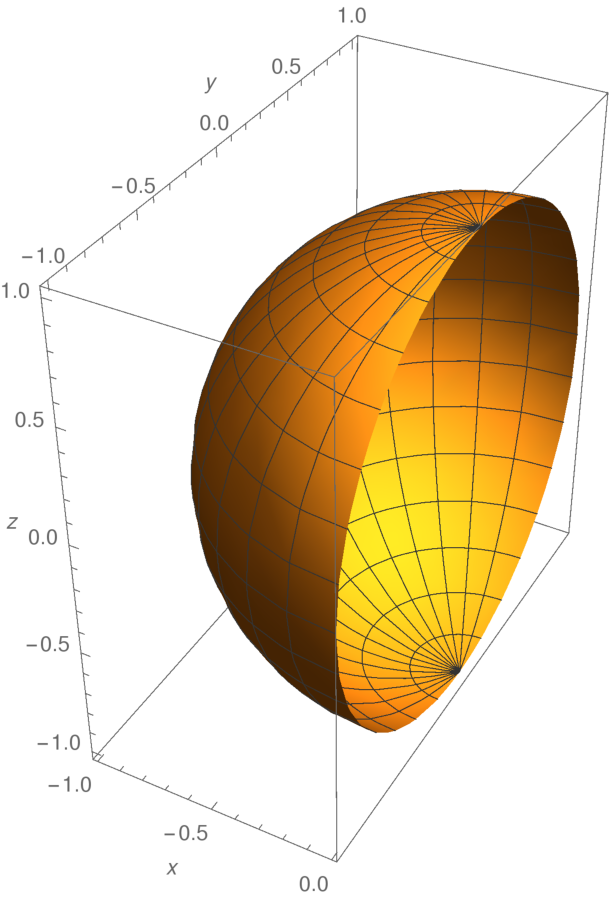
\includegraphics[width=.3\linewidth]{x-minus.pdf}
    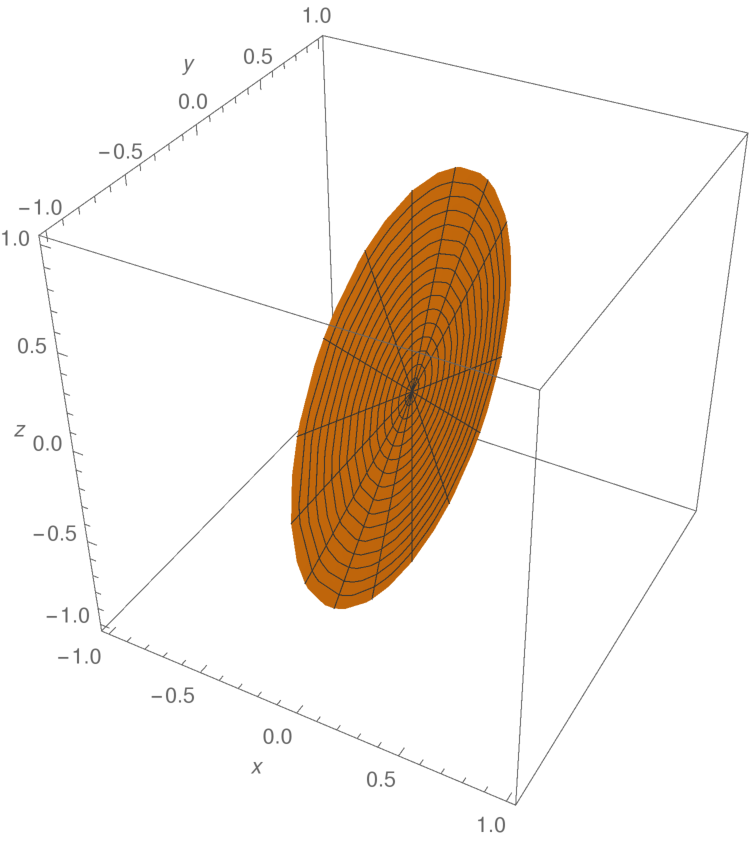
\includegraphics[width=.3\linewidth]{domain-x.pdf}
    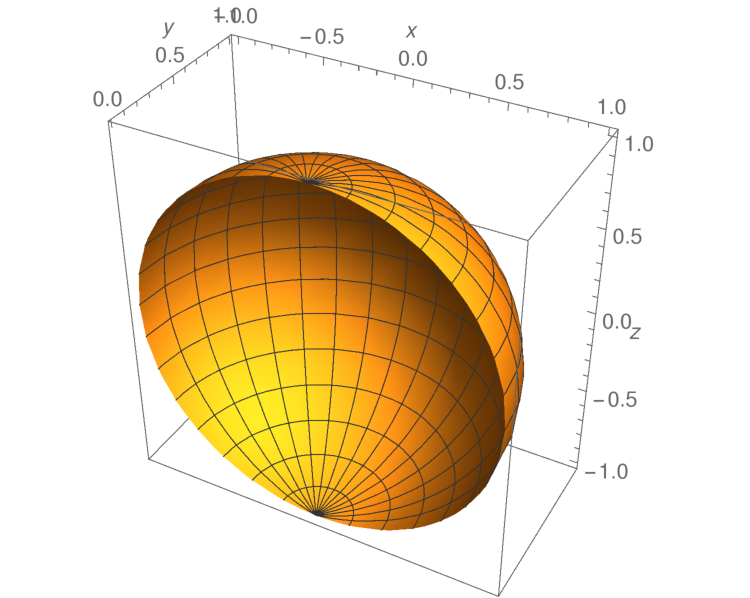
\includegraphics[width=.3\linewidth]{y-plus.pdf}
    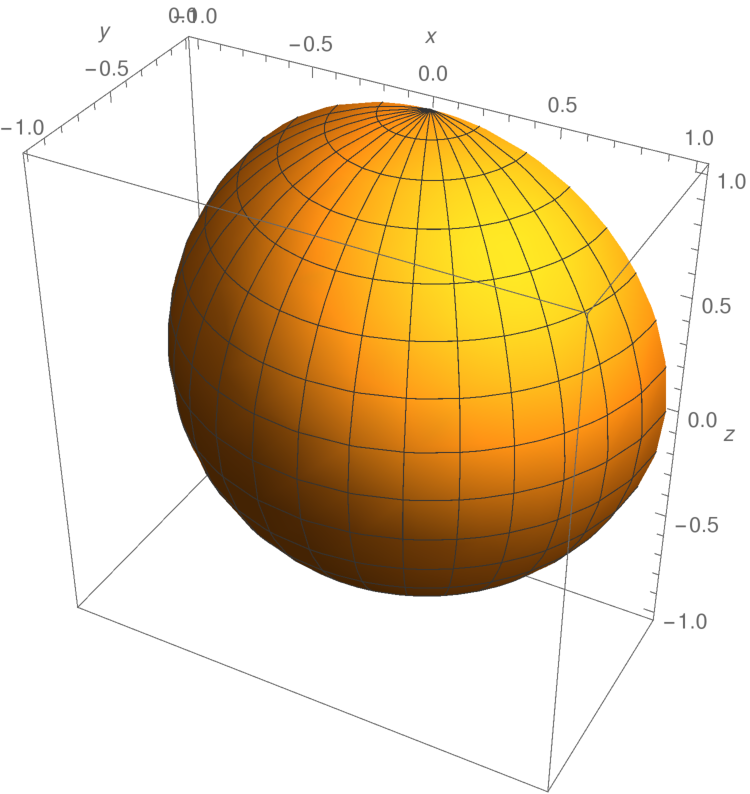
\includegraphics[width=.3\linewidth]{y-minus.pdf}
    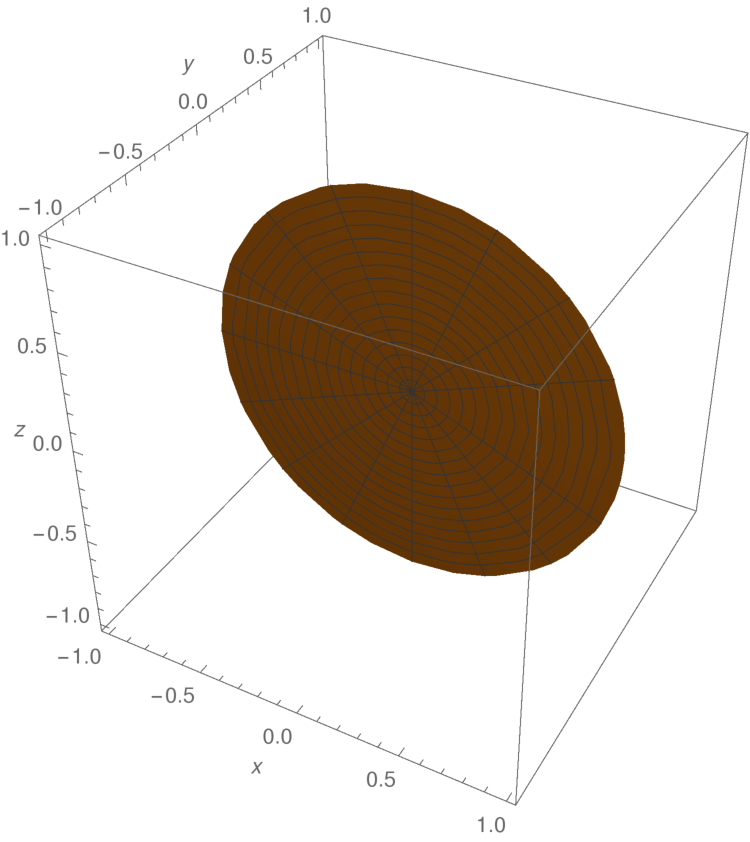
\includegraphics[width=.3\linewidth]{domain-y.pdf}
    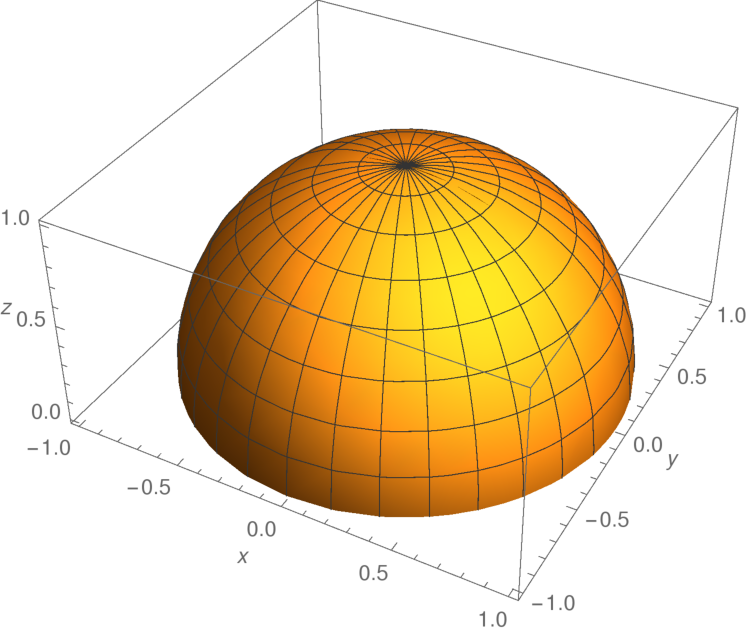
\includegraphics[width=.3\linewidth]{z-plus.pdf}
    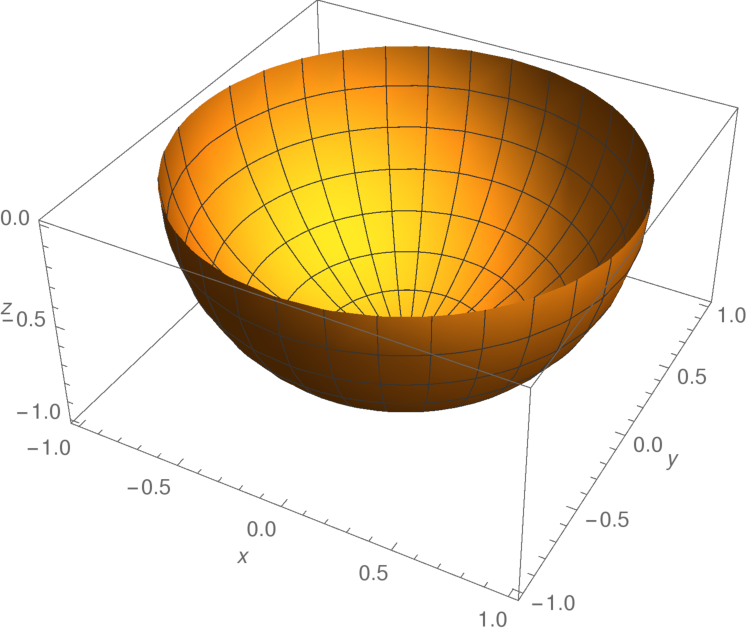
\includegraphics[width=.3\linewidth]{z-minus.pdf}
    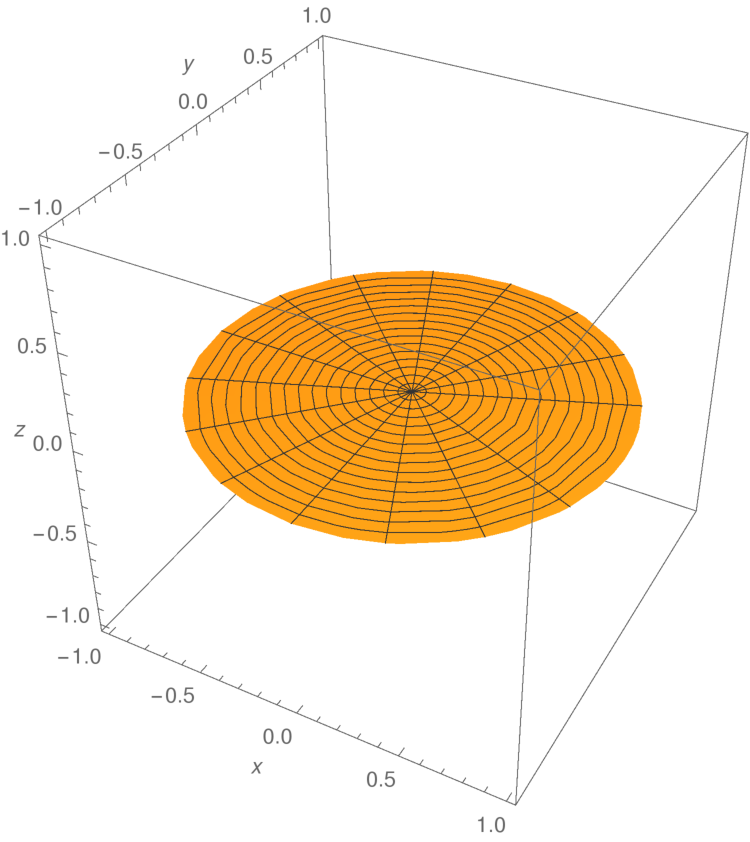
\includegraphics[width=.3\linewidth]{domain-z.pdf}
    \caption{%
        Domains and images of the charts $(\alpha_i^\pm, U_i^\pm)$. Top is $i =
        1$, middle $i = 2$ and bottom $i = 3$. The left column shows the domain
        of the “$+$” branch, the middle column shows the image of the “$-$”
        branch. The right column shows the image, which is the same for both
        branches.
    }
    \label{fig:domains}
\end{figure}

\subsection{Bijective and continuous}

$\alpha_1^+$ is surjective.

\begin{proof}
    We have to show that
    \[
        \forall \vec y \in D_1^2 \colon \exists \vec x \in U_1^+ \colon
        \alpha_1^+(\vec x) = \vec y.
    \]
    We insert $\alpha_1^+$ and write out the vectors:
    \[
        \forall \vec y \in D_1^2 \colon \exists \vec x \in U_1^+ \colon
        (x_1, x_2, x_3)|_{x_1 = 0} = (0, y_2, y_3).
    \]
    The vector $\vec y$ is written as a $\R^3$-vector since the image seems to
    be embedded in that space for convenience. We apply the mapping completely
    and obtain:
    \[
        \forall \vec y \in D_1^2 \colon \exists \vec x \in U_1^+ \colon
        (0, x_2, x_3) = (0, y_2, y_3).
    \]
    From here, we think it should be clear that such a $\vec x$ exists and
    therefore $\alpha_1^+$ is surjective.
\end{proof}

$\alpha_1^+$ is injective.

\begin{proof}
    We have to show that
    \[
        \forall \vec x, \vec y \in U_1^+ \colon \sbr{
            \alpha_i^+(\vec x) = \alpha_i^+(\vec y)
            \implies
            \vec x = \vec y
        }.
    \]
    We again carry out the mapping and write the vectors with components:
    \[
        \forall \vec x, \vec y \in U_1^+ \colon \sbr{
            (0, x_2, x_3) = (0, y_2, y_3)
            \implies
            (x_1, x_2, x_3) = (y_1, y_2, y_3)
        }.
    \]
    Since the mapping is surjective, for any given $y_2$ and $y_3$, the missing
    $y_1$ such that $|\vec y| = 1$ can be found by $x_1 = \sqrt{1 - x_2^2 -
    x_3^2}$. Therefore, the equality in the second and third component is
    sufficient to assert that the first component must be same.
\end{proof}

Taking both facts together, we have shown that the mapping is bijective. We
still have to show that it is continuous.

\begin{proof}
    To show that a mapping is continuous, it usually is easier to use the
    $\epsilon$-$\delta$ formulation. In our case we have to show that
    \[
        \forall \epsilon > 0 \colon
        \forall \vec x \in U_1^+ \colon
        \exists \delta(\vec x) > 0 \colon
        \forall \vec x' \in U_1^+ \colon
        |\vec x - \vec x'| < \delta
        \implies
        \abs{\alpha_1^+(\vec x) - \alpha_1^+(\vec x')} < \epsilon.
    \]
    Having the $\epsilon$ in front of the $\vec x$ ($\epsilon$ independent of
    $\vec x$) means something even stronger than continuity, but we even get
    that here. We now put in our mapping and omit the quantifiers since they
    stay the same. We get:
    \[
        \abs{(x_1 - x_1', x_2 - x_2', x_3 - x_3')} < \delta
        \implies
        \abs{(0, x_2 - x_2', x_3 - x_3')} < \epsilon.
    \]
    Using $\delta := \epsilon$, this certainly is fulfilled. Therefore, the
    mapping is continuous.
\end{proof}

\section{Equivalence relations}

\subsection{Show that it is one}

\renewcommand\mod{\operatorname{mod}}

The \textbf{reflectivity} is shown quickly.
\[
    x \sim x \iff x \mod n = x \mod n
\]
is fulfilled since the equality itself obeys reflectivity.

Since the equality itself is symmetric, the \textbf{symmetry} of the
equivalence relation is shown as quick as the previous property:
\[
    x \sim y
    \iff
    x \mod n = y \mod n
    \iff
    y \mod n = x \mod n
    \iff
    y \sim x.
\]

For the \textbf{transitivity}, let $x \sim y$ and $y \sim z$. Then we use the
transitivity of the equality to show:
\begin{align*}
    x \sim y \land y \sim z
    &\iff
    x \mod n = y \mod n
    \land
    y \mod n = z \mod n \\
    &\iff
    x \mod n = y \mod n = z \mod n \\
    &\implies
    x \mod n = z \mod n \\
    &\iff
    x \sim z.
\end{align*}

\subsection{Cardinality of quotient set}

If $x \in [a]$, then by the definition of the equivalence class, we have
\[
    [a] = \set{x \in \Z \colon x \sim a}
    = \set{x \in \Z \colon x \mod n = a \mod n}.
\]
We choose the representative $a$ of the equivalence class such that
\[
    a \mod n = a
    \iff
    0 \leq a < n.
\]
Now we have
\[
    [a]
    = \set{x \in \Z \colon x \mod n = a}
    = \set{a + kn \colon k \in \Z}.
\]
The only unique $a$ are $a = 0, \ldots, n-1$ such that the number of those sets
is just $n$.

\end{document}

% vim: spell spelllang=en tw=79
